\documentclass{beamer}

\usetheme{Berlin}
%\usetheme{Ilmenau}
\usefonttheme{structurebold}

\title{The Mirai Botnet}
\author{Ulysses Butler, Torey Clark, Tung Thai, and Thu Vo}

\institute{ Truman State University \\ Binary Beasts }

\date{}

%https://www.usenix.org/system/files/conference/usenixsecurity17/sec17-antonakakis.pdf

%You are expected to read and analyze and dissect the information presented in the research paper, and if you look up online you might also be able to find PPT/Video presentation of the paper. Based on your understanding your team would prepare a research presentation that'd include the problem statement (issue), methodology (process), results including pros-cons of the research paper. You are expected to go above and beyond the assigned paper and present your "RESEARCHED" information in a concise manner about the topic.  Any sort of demo is highly encouraged but not required.

%The presentation would last 35 minutes so prepare accordingly and each team member is required to participate in presenting the material. You are also required to prepare a summary document in 800-1200 words, that presents the crux of the research problem and possible solutions. 

%Each team shall have 35 mins to present their research on their topic. You should include the problem statement, motivation, related works, background, contribution, evaluation, significance of the research paper along with your own research on the topic.

\begin{document}

\maketitle

\section{Introduction}

\begin{frame}
	\frametitle{The Paper}
	\begin{itemize}
		\item<+-> Title: \textit{Understanding the Mirai Botnet}
		\item<+-> \textit{The Proceedings of the 26th USENIX Security Symposium}
		\item<+-> This paper explores the Mirai botnet
		\item<+-> This botnet was responsible for one of the largest DDoS attacks every recorded.
		\item<+-> The purpose of this paper was to learn about how the botnet worked.
		\item<+-> Researchers from a number of institutions reversed engineered it to better understand how it spread
		\item<+-> This paper then proposes reforms that can be made to prevent this kind of attack in the future
	\end{itemize}
\end{frame}

\begin{frame}
	\frametitle{Contributions}
	\begin{itemize}
		\item<1-> Lead Author
		\begin{itemize}
			\item<1-> Zane Ma - University of Illinois Urbana-Champaign
		\end{itemize}
		\item<2-> This paper had help from many different authors
		\begin{itemize}
			\item<3-> Manos Antonakakis - Georgia Institute of Technology
			\item<3-> Tim April - Akamai Technologies
			\item<3-> Michael Bailey - University of Illinois Urbana-Champaign
			\item<3-> Matthew Bernhard - University of Michigan
			\item<3-> Elie Bursztein - Google
			\item<3-> Jaime Cochran - Cloudflare
			\item<3-> Zakir Durumeric - University of Michigan
			\item<3-> J. Alex Halderman - University of Michigan
		\end{itemize}
	\end{itemize}
\end{frame}

\begin{frame}
	\frametitle{Contributions Cont.}
	\begin{itemize}
		\item<1-> Continued...
		\begin{itemize}
			\item<1-> Luca Invernizzi - Google
			\item<1-> Michalis Kallitsis - Merit Network
			\item<1-> Deepak Kumar - University of Illinois Urbana-Champaign
			\item<1-> Chaz Lever - Georgia Institute of Technology
			\item<1-> Joshua Mason - University of Illinois Urbana-Champaign
			\item<1-> Damian Menscher - Google
			\item<1-> Chad Seaman - Akamai Technologies
			\item<1-> Nick Sullivan - Cloudflare
			\item<1-> Kurt Thomas - Google
			\item<1-> Yi Zhou - University of Illinois Urbana-Champaign
		\end{itemize}
	\end{itemize}
\end{frame}

\section{Spreading}

\begin{frame}
	\frametitle{Bootstraping}
	\begin{itemize}
		\item<+-> August 1, 2016: Servers owned by DataWagon began a preliminary scan.
		\begin{itemize}
			\item<+-> DataWagon is a bulletproof web hosting provider.
			\item<+-> Users are allowed to upload and distribute almost anything using their service.
		\end{itemize}
		\item<+-> After this scan, the botnet started infecting computers
		\begin{itemize}
			\item<+-> 1 minute -  800 infected devices
			\item<+-> 10 minutes - 11,000 infected devices
			\item<+-> 20 hours - 65,000 infected devices
			\item<+-> Held steady at around 100,000 to 200,000 infections
			\item<+-> In December 2016, it peaked at 600,000 devices before beginning to fade
		\end{itemize}
	\end{itemize}
\end{frame}

\begin{frame}
	\frametitle{Spreading}
	\begin{columns}
		\column{0.5\linewidth}
			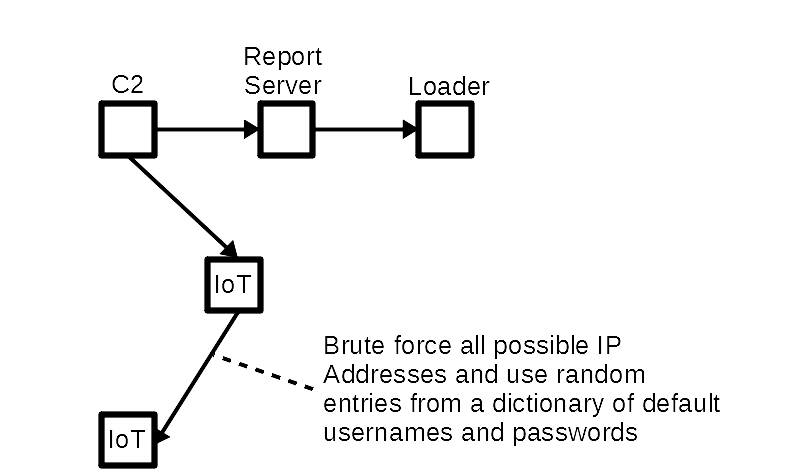
\includegraphics[width=\textwidth]{fig1.png}
		\column{0.5\linewidth}
			\begin{itemize}
				\item<+-> A member of the botnet begins scanning ports on all IPv4 addresses
				\item<+-> It scans to find open ports for SSH, Telnet, FTP, and other protocols
				\item<+-> It would then use a dictionary attack to brute force into the machine
				\item<+-> These were small dictionaries, containing 60 to about 200 credentials
			\end{itemize}
	\end{columns}
\end{frame}

\begin{frame}
	\frametitle{Spreading}
	\begin{columns}
		\column{0.5\linewidth}
			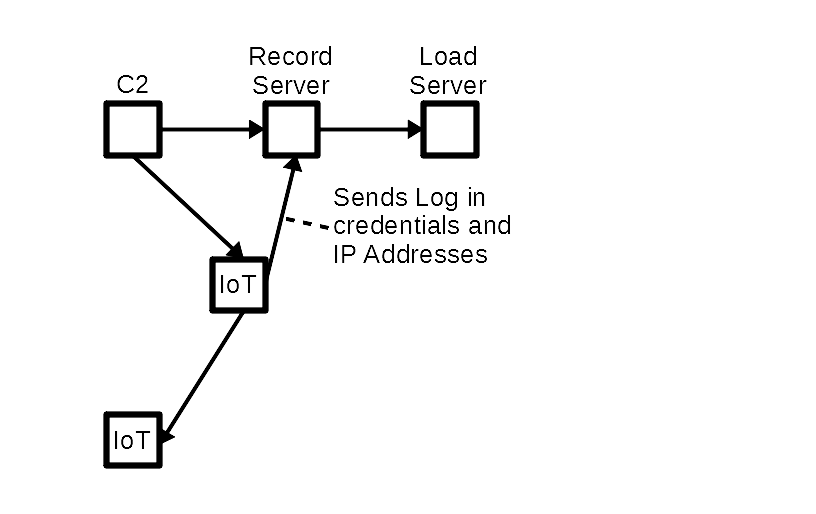
\includegraphics[width=\textwidth]{fig2.png}
		\column{0.5\linewidth}
			\begin{itemize}
				\item<+-> The address and credentials of the victim machines where then sent to a report server
				\item<+-> This information could later be used by the Command and Control (C2) server
			\end{itemize}
	\end{columns}
\end{frame}

\begin{frame}
	\frametitle{Spreading}
	\begin{columns}
		\column{0.5\linewidth}
			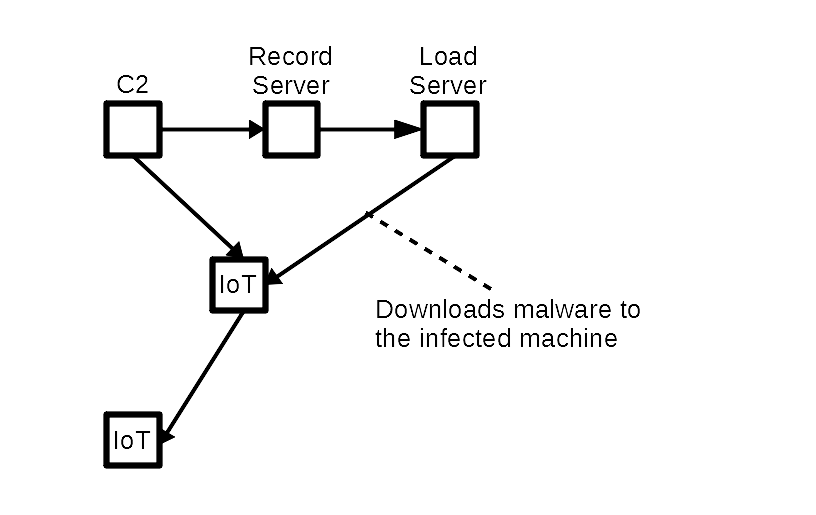
\includegraphics[width=\textwidth]{fig3.png}
		\column{0.5\linewidth}
			\begin{itemize}
				\item<+-> The records server then sent this information to the load program
				\item<+-> This program would download a binary onto the victim and run the program
			\end{itemize}
	\end{columns}
\end{frame}

\begin{frame}
	\frametitle{Loading the Binary}
	\begin{itemize}
		\item<+-> The aforementioned loader program downloaded an architecture specific binary
		\item<+-> The machine would then run the binary and change the process information to make it harder to detect
		\item<+-> The binary is then deleted.
		\begin{itemize}
			\item<+-> This means infections won't carry across reboots
		\end{itemize}
		\item<+-> Once the victim is infected, it starts scanning
		\begin{itemize}
			\item<+-> It would specifically avoid scanning servers owned by major corporations or the government
			\item<+-> These entities would likely be too secure for this simple attack
			\item<+-> This also allowed the bot to keep a lower profile
			\item<+-> These organizations would be much more likely to start search for and exploiting weaknesses in the malware if it infected their machines
		\end{itemize}
	\end{itemize}
\end{frame}

\section{Exploiting IoT}

\begin{frame}[fragile]
	\frametitle{Internet of Things Security}
	\begin{itemize}
		\item<+-> The Internet of Things
		\begin{itemize}
			\item<+-> Includes security cameras, routers, network-access storage, TV receivers, printer, DVRs, etc.
			\item<+-> Typically embedded systems that aren't powerful
		\end{itemize}
		\item<+-> Manufactures neglect security
		\begin{itemize}
			\item<+-> Many manufactures use one user name and password
			\item<+-> Common passwords are frequent. \verb|password|, \verb|admin|, etc.
			\item<+-> Some devices even have credentials hard coded in firmware
			\item<+-> Most companies don't have the infrastructure to release patches for these systems
		\end{itemize}
		\item<+-> This allowed the bot to easily infect a large number of machines
	\end{itemize}
\end{frame}

\begin{frame}
	\frametitle{Disadvantages}
	\begin{itemize}
		\item<+-> These less powerful devices also hurt Mirai's growth
		\begin{itemize}
			\item<+-> Mirai had a doubling time of 75-minutes
			\begin{itemize}
				\item<+-> Compare to 37-minutes for Code-Red
				\item<+-> 9-minutes for Blaster
			\end{itemize}
			\item<+-> Most bots scanned at less than 250 bytes per second
			\item<+-> Much slower than other bot nets
			\item<+-> SQL Slammer was about 6000 times faster at 1.5 megabytes per second
		\end{itemize}
		\item<+-> Most devices were found in low bandwidth countries
		\begin{itemize}
			\item<+-> Most infected devices were from South America and South-east Asia
			\item<+-> Brazil, Colombia, and Vietnam hosted most of the bots
		\end{itemize}
	\end{itemize}
\end{frame}

\section{Attacking}

\begin{frame}
    \frametitle{How DDoS Works}
    \begin{itemize}
        \item How to DDoS for Dummies
            \begin{itemize}
                \item<+-> A DDoS seeks to restrict a servers capabilities to respond to users by flooding it with requests from multiple different machines.
                \item<+-> DDoS attacks are more difficult to protect against compared to a DoS attack
                \item<+-> It is difficult to blacklist multiple IP Addresses
                \item<+-> It's nearly impossible to distinguish between real requests and the attack.
            \end{itemize}
    \end{itemize}
\end{frame}

\begin{frame}
    \frametitle{Volumetric Attacks}
        \begin{itemize}
            \item<+-> Volumetric Attacks consist of a flooding a server with request packets
            \item<+-> Overwhelms its ability to respond
            \item<+-> Requires work to generate a high count of requests
            \item<+-> With requests from multiple machines, it is difficult to prevent or dampen an attack on a server.
    \end{itemize}
\end{frame}
\begin{frame}
    \frametitle{Protocal Attacks}
     \begin{itemize}
            \item<+-> Protocol Attacks seek to disable a server by exploiting a weakness in a given protocol
            \item<+-> SYN floods attacks TCP by exploiting the three-way handshake process to create a backlogged queue
            \item<+-> Ping attacks uses a large number of pings to attack a server
            \item<+-> UDP floods send massive amounts of packets to random ports to overwhelm the queue of responses
        \end{itemize}
\end{frame}

\begin{frame}
    \frametitle{Application Layer Attacks}
        \begin{itemize}
            \item<+-> Application layer attacks attempt to exploit the layer of human interaction with a machine
            \item<+-> Nearly indistinguishable from real user interaction
            \item<+-> requires far less resources to execute this attack than it takes to prevent that attack
            \item<+-> This makes these attacks resource efficient for an attacker
    \end{itemize}
\end{frame}

\begin{frame}
    \frametitle{Types of Services Attacked}
    \begin{itemize}
        \item<+-> Most attacks were orchestrated against targets in the United States(50.3\%), France(6.6\%), and the UK(6.1\%).
        \item<+-> Mirai could also target particular ports to affect specific services
        \begin{itemize}
        		\item<+-> The most common ones attacked were 80(HTTP, 37.5\%)
        		\item<+-> 25565(Minecraft, 9.2\%)
        		\item<+-> 443(HTTPS, 6.4\%)
        		\item<+-> and 23594(Runescape, 3.4\%)
        \end{itemize}
        \item<+-> Several Mirai C2 servers were attacked by some of its other C2 servers
        \item<+-> These were likely from renting DDoS attackers against other renting DDoS attackers.
    \end{itemize}
\end{frame}

\begin{frame}
    \frametitle{Attacks}
	\begin{itemize}
		\item<+-> General Targets by Mirai
			\begin{itemize}
				\item<+-> Multiple DDoS attacks against a variety of targets
				\item<+-> Game Servers (primarily Minecraft and Runescape)
				\item<+-> Political WebsitesA
				\item<+-> Anti-DDoS services
			\end{itemize}
		\item<+-> Notable Targets
			\begin{itemize}
				\item<+-> Krebs on Security
				\begin{itemize}
					\item<+-> This was a high-profile attack on a well-known security blog
					\item<+-> The attack peaked at around 600 Gbps, the largest Akamai had ever seen 						\item<+-> This forced them to drop Krebs as a client due to high costs
				\end{itemize}
				\item<+-> Dyn - DNS attack disrupted access for Amazon, Github, Netflix, Twitter, and others
				\item<+-> Lonestar Cell - most attacked target, destroyed internet capabilities in Liberia
			\end{itemize}
	\end{itemize}
\end{frame}

\section{Methodology}

\begin{frame}
	\frametitle{Methodology}
	\begin{itemize}
		\item<+-> The researches and authors of this paper used a number of techniques
		\item<+-> They used attempted to monitor the botnet's spread
		\item<+-> Many binaries used by the malware were captured
		\item<+-> A number of organizations tried a variety of techniques and shared their information for this paper.
	\end{itemize}
\end{frame}

\begin{frame}
	\frametitle{Network Telescope}
	\begin{itemize}
		\item<+-> One method for monitoring the spread was by using network telescopes
		\item<+-> Purpose: to analyze the growth and size of the botnet
		\item<+-> Monitored network request (scan) to a network telescope composed 4.7 millions IP address
		\begin{itemize}
			\item<+-> On average, the network telescope received 1.1 million packets from 269,000 IP addresses per minute 
			\item<+-> Observed 116.2 billions Mirai probes from 55.4 millions IP address
		\end{itemize}
		\item<+-> A raw count of IP addess is a poor metric due to DHCP churn
		\begin{itemize}
			\item<+-> Consider the number of hosts actively "scanning" at the start of every hours
			\item<+-> Identified scans that targeted the IPv4 address space at an estimated rate of at least five packets per second
		\end{itemize}
	\end{itemize}
\end{frame}

\begin{frame}
	\frametitle{Active Scanning}
	\begin{itemize}
		\item<+-> The researches also tried scanning infected devices
		\item<+-> Purpose: to analyze infected device composition (manufacturer and model).
		\item<+-> Focus on scans of HTTPS, FTP, SSH, Telnet, and CWMP.
		\item<+-> Difficulties and challenges to make accurate device labeling:		
		\begin{itemize}
			\item<+-> Mirai prevents infected devices from being scanned
			\item<+-> The scan often takes 24 hours to complete, during which devices may churn to a new IP address
			\item<+-> Resolution: restricting analysis to banners that were collected within twenty minutes of scanning activity
		\end{itemize}
		\item<+-> Post-filtering, the dataset include 1.8 millions banner associated with 1.2 million IP address
		\begin{itemize}
			\item<+-> Process each banner to identify the device manufacturer and model using Nmap
			\item<+-> In total, identified 31.5 \% of banners (about 600k banners)
		\end{itemize}
	\end{itemize}
\end{frame}

\begin{frame}
	\frametitle{Telnet Honeypots}
	\begin{itemize}
		\item<+-> Use a set of Telnet honeypots that masqueraded as vulnerable IoT
		\begin{itemize}
			\item<+-> The honeypot logged all incoming traffic and downloaded any binaries that the attackers attemps to install
			\item<+-> Block all outgoing request to avoid collateral damages
		\end{itemize}
		\item<+-> Logged 80K connection attempts from 54K IP addresses and collected 141 unique binaries.
		\begin{itemize}
			\item<+-> Supplemented these data with unique binaries from others
			\item<+-> In totals, they collected 1028 unique binaries
		\end{itemize}
		\item<+-> Analyzed the most common, binaries for MIPS 32-bit, ARM 32-bit, and x86 32-bit.
		\begin{itemize}
			\item<+-> Extracted the set of logins, password, IP blacklists, and C2 domains
			\item<+-> Identified 67 C2 domains and 48 distinct username password dictionaries (containing a total 371 unique passwords)
		\end{itemize}
	\end{itemize}
\end{frame}

\begin{frame}
	\frametitle{Active \& Passive DNS}
	\begin{itemize}
		\item<+-> Purpose: to construct a graph reflecting the shared infrastructure used by Mirai
		\item<+-> Collected 209 millions passive DNS record per day (historical record of DNS zone) and 290 millions active DNS record per day of C2 server
		\item<+-> Use above dataset to identify shared DNS infrastructure by linking related historic domain names (RHDN) and related historic IPs (RHIPs)
		\begin{itemize}
			\item<+-> For a given C2 domain, identify the IP address it previously resolved to and added them to a growing set of domains and IPs
			\item<+-> Starting from an IP and finding any domain names that concurrently resolved it
			\item<+-> In the end, from a single domain name, we can expand a set of domain name and IP addresses
		\end{itemize}
	\end{itemize}
\end{frame}

\begin{frame}
	\begin{figure}
		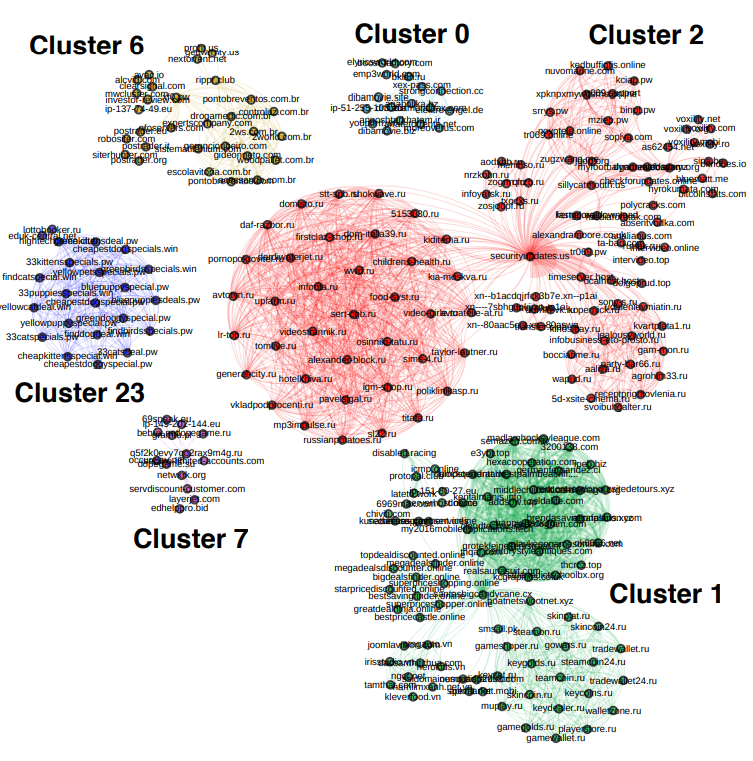
\includegraphics[width=50 mm, scale = 0.5]{C2DomainRelationship.png}
		\caption{ \textbf{C2 Domain Relationships} -- We visualize related C2 infrastructure, depicting C2 domains as nodes and shared IPs as edges between two domains.}
	\end{figure}
\end{frame}

\begin{frame}
	\frametitle{Attack Commands}
	\begin{itemize}
		\item<+-> Purpose: to track the attack commands issued by the Mirai operators
		\item<+-> Simulated a Mirai-infected device and communicated with the C2 server using a custom bot-to-C2 protocol
		\item<+-> In total, Akamai observed 64K attack commands issued by 484 unique C2 servers  (by IP address)
		\begin{itemize}
			\item<+-> This is a naive analysis because individual C2 servers often repeat the same attack command in rapid succession
			\item<+-> Resolution: collapse matching commands that occur within 90 seconds of each others
			\item<+-> Results: 15,194 attacks from 146 unique IP clusters, which cover the Dyn attack and Liberia attacks
		\end{itemize}
	\end{itemize}
\end{frame}

\begin{frame}
	\frametitle{DDoS Attack trace}
	\begin{itemize}
		\item<+-> Purpose: to corroborate the IP addresses observed in attacks versus those found scanning our network telescope.
		\begin{itemize}
			\item<+-> Dyn provided 107.5K IP addresses associated
with attack on October 21, 2016 and 158.8K IP addresses involved in attack on September 25, 2016
			\item<+-> Form a statistics to calculate what fraction of these IP addresses matched the list of IP address obseved by our network telescope
		\end{itemize}
	\end{itemize}
\end{frame}

\section{Open Source}

\begin{frame}
	\frametitle{Releasing the Source Code}
	\begin{itemize}
		\item<+-> The source code was released on September 30, 2016
		\item<+-> A user named ``Anna-senpai'' released the source code for free on hackerforums.net
		\item<+-> This spawned a number of copycat attacks with variations on the original bot
		\begin{itemize}
			\item<+-> Many included new exploits, modified dictionaries, and different IP blacklists
		\end{itemize}
		\item<+-> These botnets eventually starting competing
		\begin{itemize}
			\item<+-> Killing processes started by similar bots
			\item<+-> Closing the ports used to attack the machine
			\item<+-> At various points, competing command and control servers were subject to DDoS attacks
		\end{itemize}
	\end{itemize}
\end{frame}

\section{Defending}
\begin{frame}
    \frametitle{Defense Against the Dark Arts}
    \begin{itemize}
        \item<+-> Industry Improvements
            \begin{itemize}
                \item<+-> Randomized default passwords 
                \item<+-> Closed ports on default
                \item<+-> Employ Automatic Updates and Self-Monitoring
                \item<+-> Creating Standard for Model and Firmware identification
            \end{itemize}
        \item<+-> User Improvements
            \begin{itemize}
                \item<+-> Create good secure credentials and not use the defaults
                \item<+-> Purchase from reputable and secure companies
                \item<+-> Replace old and unsupported devices
            \end{itemize}
    \end{itemize}
\end{frame}

\begin{frame}
    \frametitle{Defense Against the Dark Arts}
    \begin{itemize}
        \item Randomized default passwords prevent attackers from employing a dictionary of default passwords.
        \item Having ports not used default to closed mitigates the chances of a successful attack.
        \item Automatic updates prevent users from refusing updates during hours of use and keeps systems secure against previous exploits. Bug bounties encourage the community to find and report all possible exploits to be patched.
        \item Standards for model and version identification allow server admins to easily see any and all machines that have known vulnerabilities.
    \end{itemize}
\end{frame}
\begin{frame}
    \frametitle{Defense Against the Dark Arts}
    \begin{itemize}
        \item Users should create secure usernames and passwords for all devices to mitigate the chance of it being hacked using brute force.
        \item Smart purchases from known and trusted companies that prioritize security of their manufactured devices acts as a deterrent from would be attackers.
        \item Old and unsupported devices should be replaced with newer models that conform with current security standards and have strong customer support.
    \end{itemize}
    
\end{frame}

\section{Further Research}

\begin{frame}
	\frametitle{Origin of Mirai}
	\begin{itemize}
		\item<+-> After this paper was released, we started to learn more about the botnet's origins
		\item<+-> Mirai was created by 3 computer science students
		\begin{itemize}
			\item<+-> 21-year-old Paras Jha
			\item<+-> 20-year-old Josiah White
			\item<+-> 21-year-old Dalton Norman
		\end{itemize}
		\item<+-> It's likely named after the anime Mirai Nikki (Future Diary)
		\item<+-> As revealed after the trial, this botnet was originally created to DDoS Minecraft servers
		\item<+-> The group allegedly started trying to profit from their botnet
		\begin{itemize}
			\item<+-> Extorting profitable servers
			\item<+-> Creating a company to protect server owners from DDoS attacks
			\item<+-> Renting out their botnet to other cybercriminals
		\end{itemize}
	\end{itemize}
\end{frame}

\begin{frame}
	\frametitle{Investigations}
	\begin{itemize}
		\item<+-> Anna-senpai boosted about his programming skills on the forum
		\begin{itemize}
			\item<+-> After investigating companies related to DataWagon, Krebs found ProTraf solutions
			\item<+-> The skills Anna-senpai had were extremely similar to Jha's.
			\item<+-> He also has experience running Minecraft servers, similar to the original targets
		\end{itemize}
		\item<+-> According to Krebs on Security, the creators then released the source code to ``distance themselves from their creation''
		\item<+-> Many attacks, such as the attack on Dyn, are believed to be a result of copy cat attackers
	\end{itemize}
\end{frame}

\begin{frame}
	\frametitle{Investigation}
	\begin{itemize}
		\item<+-> On December 8, 2017, the FBI announced that it had secured guilty pleas
		\item<+-> The authors were able to avoid jail time after cooperating with the FBI to help track other cybercriminals.
		\item<+-> This allowed them to avoid jail time
		\begin{itemize}
			\item<+-> Five-year probation
			\item<+-> 2,500 Hours of community service
			\item<+-> \$127,000 in restitution
			\item<+-> They had to forfeit the concurrency made during that time
			\item<+-> This was about 17 bitcoin
		\end{itemize}
	\end{itemize}
\end{frame}

\section{Conclusion}

\begin{frame}
	\frametitle{Conclusion}
	\begin{itemize}
		\item<+-> Mirai was a centralized botnet that was responsible for some of the largest DoS attacks every recorded.
		\item<+-> This bot was relatively simple with small dictionaries
		\item<+-> They creators of this bot exploited the security negligence of hardware manufactures
		\item<+-> They were able to quickly take over a large number of IoT devices
		\item<+-> This attack served as a wake up call, prompting reform in these industries
	\end{itemize}
\end{frame}

\end{document}
